%  The AAU Poster Theme.
%  2013-05-08 v. 1.1.0
%  Copyright 2013 by Jesper Kjær Nielsen <jkn@es.aau.dk>
%
%  This is free software: you can redistribute it and/or modify
%  it under the terms of the GNU General Public License as published by
%  the Free Software Foundation, either version 3 of the License, or
%  (at your option) any later version.
%
%  This is distributed in the hope that it will be useful,
%  but WITHOUT ANY WARRANTY; without even the implied warranty of
%  MERCHANTABILITY or FITNESS FOR A PARTICULAR PURPOSE.  See the
%  GNU General Public License for more details.
%
%  You can find the GNU General Public License at <http://www.gnu.org/licenses/>.
\documentclass[a0paper,portrait]{baposter}
%%%%%%%%%%%%%%%%%%%%%%%%%%%%%%%%%%%%%%%%%%%%%%%%
% Language, Encoding and Fonts
% http://en.wikibooks.org/wiki/LaTeX/Internationalization
%%%%%%%%%%%%%%%%%%%%%%%%%%%%%%%%%%%%%%%%%%%%%%%%
% Select encoding of your inputs. Depends on
% your operating system and its default input
% encoding. Typically, you should use
%   Linux  : utf8 (most modern Linux distributions)
%            latin1
%   Windows: ansinew
%            latin1 (works in most cases)
%   Mac    : applemac
% Notice that you can manually change the input
% encoding of your files by selecting "save as"
% an select the desired input encoding.
\usepackage[utf8]{inputenc}
% Make latex understand and use the typographic
% rules of the language used in the document.
\usepackage[english]{babel}
% Use the vector font Latin Modern which is going
% to be the default font in latex in the future.
\usepackage{helvet}
% Change the default font family from roman to sans serif
\renewcommand{\familydefault}{\sfdefault} % for text
\usepackage[helvet]{sfmath} % for math
% Choose the font encoding
\usepackage[T1]{fontenc}

%%%%%%%%%%%%%%%%%%%%%%%%%%%%%%%%%%%%%%%%%%%%%%%%
% Graphics and Tables
% http://en.wikibooks.org/wiki/LaTeX/Importing_Graphics
% http://en.wikibooks.org/wiki/LaTeX/Tables
% http://pgfplots.sourceforge.net/
%%%%%%%%%%%%%%%%%%%%%%%%%%%%%%%%%%%%%%%%%%%%%%%%
% You cannot use floats in the baposter theme.
% We therefore load the caption package which provides
% the command \captionof
% Set up how figure and table captions are displayed
\usepackage{caption}
\captionsetup{
  font=small,% set font size to footnotesize
  labelfont=bf % bold label (e.g., Figure 3.2) font
}
% Make the standard latex tables look so much better
\usepackage{array,booktabs}
% For creating beautiful plots
\usepackage{pgfplots}

%%%%%%%%%%%%%%%%%%%%%%%%%%%%%%%%%%%%%%%%%%%%%%%%
% Mathematics
% http://en.wikibooks.org/wiki/LaTeX/Mathematics
%%%%%%%%%%%%%%%%%%%%%%%%%%%%%%%%%%%%%%%%%%%%%%%%
% Defines new environments such as equation,
% align and split
\usepackage{amsmath}
% Adds new math symbols
\usepackage{amssymb}

%%%%%%%%%%%%%%%%%%%%%%%%%%%%%%%%%%%%%%%%%%%%%%%%
% Colours
% http://en.wikibooks.org/wiki/LaTeX/Colors
%%%%%%%%%%%%%%%%%%%%%%%%%%%%%%%%%%%%%%%%%%%%%%%%
\selectcolormodel{RGB}
% define the three aau colors
\definecolor{aaublue1}{RGB}{33,26,82}% dark blue
\definecolor{aaublue2}{RGB}{113,109,143} % light blue
\definecolor{aaublue3}{RGB}{194,193,204} % lighter blue

%%%%%%%%%%%%%%%%%%%%%%%%%%%%%%%%%%%%%%%%%%%%%%%%
% Lists
% http://en.wikibooks.org/wiki/LaTeX/List_Structures
%%%%%%%%%%%%%%%%%%%%%%%%%%%%%%%%%%%%%%%%%%%%%%%%
% Easier configuration of lists
\usepackage{enumitem}
%configure itemize
\setlist{%
  topsep=0pt,% set space before and after list
  noitemsep,% remove space between items
  labelindent=\parindent,% set the label indentation to the paragraph indentation
  leftmargin=*,% remove the left margin
  font=\color{aaublue1}\normalfont, %set the colour of all bullets, numbers and descriptions to aaublue1
}
% use set<itemize,enumerate,description> if you have an older latex distribution
\setitemize[1]{label={\raise1.25pt\hbox{$\blacktriangleright$}}}
\setitemize[2]{label={\scriptsize\raise1.25pt\hbox{$\blacktriangleright$}}}
\setitemize[3]{label={\raise1.25pt\hbox{$\star$}}}
\setitemize[4]{label={-}}
%\setenumerate[1]{label={\theenumi.}}
%\setenumerate[2]{label={(\theenumii)}}
%\setenumerate[3]{label={\theenumiii.}}
%\setenumerate[4]{label={\theenumiv.}}
%\setdescription{font=\color{aaublue1}\normalfont\bfseries}

% use setlist[<itemize,enumerate,description>,<level>] if you have a newer latex distribution
%\setlist[itemize,1]{label={\raise1.25pt\hbox{$\blacktriangleright$}}}
%\setlist[itemize,2]{label={\scriptsize\raise1.25pt\hbox{$\blacktriangleright$}}}
%\setlist[itemize,3]{label={\raise1.25pt\hbox{$\star$}}}
%\setlist[itemize,4]{label={-}}
%\setlist[enumerate,1]{label={\theenumi.}}
%\setlist[enumerate,2]{label={(\theenumii)}}
%\setlist[enumerate,3]{label={\theenumiii.}}
%\setlist[enumerate,4]{label={\theenumiv.}}
%\setlist[description]{font=\color{aaublue1}\normalfont\bfseries}

%%%%%%%%%%%%%%%%%%%%%%%%%%%%%%%%%%%%%%%%%%%%%%%%
% Misc
%%%%%%%%%%%%%%%%%%%%%%%%%%%%%%%%%%%%%%%%%%%%%%%%
% change/remove some names
\addto{\captionsenglish}{
  %remove the title of the bibliograhpy
  \renewcommand{\refname}{\vspace{-0.7em}}
  %change Figure to Fig. in figure captions
  \renewcommand{\figurename}{Fig.}
}
% create links
\usepackage{url}
%note that the hyperref package is currently incompatible with the baposter class

%%%%%%%%%%%%%%%%%%%%%%%%%%%%%%%%%%%%%%%%%%%%%%%%
% Macros
%%%%%%%%%%%%%%%%%%%%%%%%%%%%%%%%%%%%%%%%%%%%%%%%
\newcommand{\alert}[1]{{\color{aaublue1}#1}}

%%%%%%%%%%%%%%%%%%%%%%%%%%%%%%%%%%%%%%%%%%%%%%%%
% Document Start
%%%%%%%%%%%%%%%%%%%%%%%%%%%%%%%%%%%%%%%%%%%%%%%%
\begin{document}
%%%%%%%%%%%%%%%%%%%%%%%%%%%%%%%%%%%%%%%%%%%%%%%%
% Some changes that cannot be made in the preamble
%%%%%%%%%%%%%%%%%%%%%%%%%%%%%%%%%%%%%%%%%%%%%%%%
% set the background of the poster
\background{
  \begin{tikzpicture}[remember picture,overlay]%
    %the poster background color
    \fill[fill=aaublue3] (current page.north west) rectangle (current page.south east);
    %the header
    \fill [fill=aaublue1] (current page.north west) rectangle ([yshift=-\headerheight] current page.north east);
  \end{tikzpicture}
}
% if you want to reduce the space before and after equations, use and adjust
% the following lines
%\addtolength{\abovedisplayskip}{-2mm}
%\addtolength{\belowdisplayskip}{-2mm}

%%%%%%%%%%%%%%%%%%%%%%%%%%%%%%%%%%%%%%%%%%%%%%%%
% General poster setup
%%%%%%%%%%%%%%%%%%%%%%%%%%%%%%%%%%%%%%%%%%%%%%%%
\begin{poster}{
  %general options for the poster
  grid=false,
  columns=3,
%  colspacing=4.2mm,
  headerheight=0.1\textheight,
  background=user,
%  bgColorOne=red!42, %is used when background != user and none
%  bgColortwo=green!42, %is used when background is shaded
  eyecatcher=true,
  %posterbox options
  headerborder=closed,
  borderColor=aaublue1,
  headershape=rectangle,
  headershade=plain,
  headerColorOne=aaublue1,
%  headerColortwo=yellow!42, %is used when the header background is shaded
  textborder=rectangle,
  boxshade=plain,
  boxColorOne=white,
%  boxColorTwo=cyan!42,%is used when the text background is shaded
  headerFontColor=white,
  headerfont=\Large\sf\bf,
  linewidth=1pt
}
%the Eye Catcher (the logo on the left)
{
  %this can be commented out or replaced by a company/department logo
  
\includegraphics[height=0.75\headerheight]{pku_neg}
}
%the poster title
{\color{white}\bf
  Text Detection and Localization \\from Complex Background
}
%the author(s)
{\color{white}\bf
  \vspace{0.2em} Mingmin Zhao, Yisong Chen\\[0.2em]
  \color{white}\small
  Key Lab. of Machine Perception (MoE), Peking University, Beijing, China\\
  zhaomingmin@pku.edu.cn
}
%the logo (the logo on the right)
{
  %this can be commented out or replaced by a company/department logo
  
\includegraphics[height=0.75\headerheight]{pku_neg}
}








%%%%%%%%%%%%%%%%%%%%%%%%%%%%%%%%%%%%%%%%%%%%%%%%
% the actual content of the poster begins here
%%%%%%%%%%%%%%%%%%%%%%%%%%%%%%%%%%%%%%%%%%%%%%%%

\begin{posterbox}[name=overview,column=0,row=0]{Overview}
\begin{itemize}
  \item Text in images and video frames is one of the most powerful sources of high-level semantics once the text can be detected, localized and recognized automatically.
  \item In this paper, we develop a two-stage method to detect and locate text lines from complex background.
  \item The experiment on challenging datasets from ICDAR shows that this is a fast and robust method to detect and locate text lines in complex background.
\end{itemize}
\end{posterbox}









\begin{posterbox}[name=method,column=0,below=overview]{Our Method}
\begin{itemize}
  \item A coarse-to-fine two-stage architecture
  \item At the coarse stage, our method use several basic features of text to select candidate text lines.
  \item At the fine stage, using candidates from the first stage as input, an SVM classifier based on HOG feature and co-occurrence matrix features identify true text lines from candidates.
\end{itemize}
\end{posterbox}










\begin{posterbox}[name=text,column=0,below=method]{Properties of Text}

\begin{itemize}
  \item Edge:
    \begin{itemize}
      \item Most texts are designed to be striking and easily read.
      \item Thereby resulting in strong edges at the boundaries of text and background.
    \end{itemize}
  \item Color:
    \begin{itemize}
        \item Every single character tends to have the same or similar color.
    \end{itemize}
  \item Edge:
    \begin{itemize}
        \item Texts appear in clusters.
        \item Characters within a text line tend to have similar size and are always aligned.
    \end{itemize}
\end{itemize}

\end{posterbox}











\begin{posterbox}[name=pipeline,column=0,below=text,above=bottom]{Pipeline of Coarse Detection}
The goal of coarse detection is to find text-like textures from original image.\\
We developed a method to find text-like textures as follow:\\
%\begin{equation}
%  f_X(x|\mu,\sigma^2) = \frac{1}{\sqrt{2\pi\sigma^2}}\exp\left\{\frac{1}{2\sigma^2}(x-\mu)^2\right\}
%\end{equation}
\begin{center}
  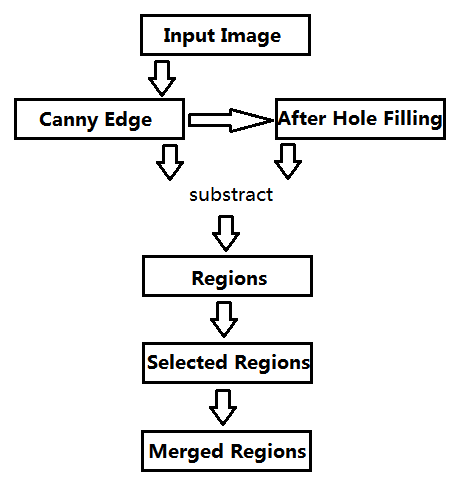
\includegraphics[width=1.8\headerheight]{pipeline}
  \captionof{figure}{Pipeline of coarse detection}
  \label{fig:figlabel}
\end{center}

\end{posterbox}


















\begin{posterbox}[name=example,span=2,column=1,row=0]{Coarse Detection}
\begin{center}
  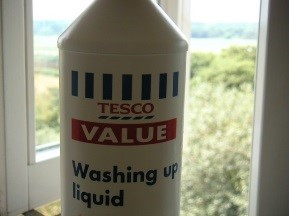
\includegraphics[width=1.45\headerheight]{step1.jpg}
  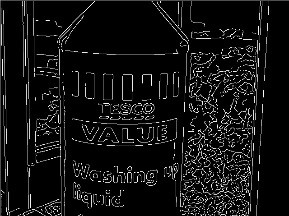
\includegraphics[width=1.45\headerheight]{step2.jpg}
  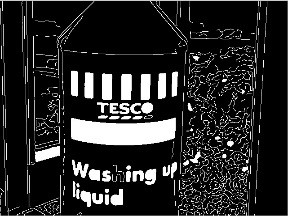
\includegraphics[width=1.45\headerheight]{step3.jpg}
  \vspace{0.3cm}
  \hfill
  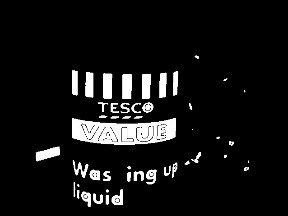
\includegraphics[width=1.45\headerheight]{step4.jpg}
  
\includegraphics[width=1.45\headerheight]{step5.jpg}
  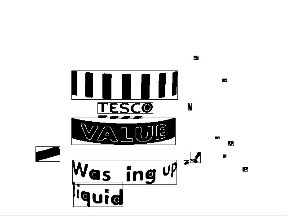
\includegraphics[width=1.45\headerheight]{step6.jpg}
  \captionof{figure}{An example of coarse detection}
  \label{fig:figlabel}
\end{center}
\end{posterbox}






\begin{posterbox}[name=feature,column=1,below = example]{Features for Fine Detection}

\begin{itemize}
  \item HOG features after splitting:
    \begin{center}
    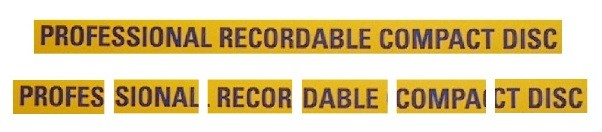
\includegraphics[width=1.8\headerheight]{split.jpg}
    \captionof{figure}{An example of splitting}
    \label{fig:figlabel}
    \end{center}

  \item Co-occurrence Matrix features:
  \begin{itemize}
    \item Statistics:
    \begin{equation}
        Contrast: \sum_{i,j} |i-j|^2 p(i,j)
    \end{equation}
    \begin{equation}
        Correlation: \sum_{i,j} \frac{(i-\mu_i)(j-\mu_j)p(i,j)}{\sigma_i\sigma_j}
    \end{equation}
    \begin{equation}
        Energy: \sum_{i,j} p(i,j)^2
    \end{equation}
    \begin{equation}
        Homogeneity: \sum_{i,j} \frac{p(i,j)}{1+|i-j|}
    \end{equation}

    \item Different offsets are used:
    \begin{center}
        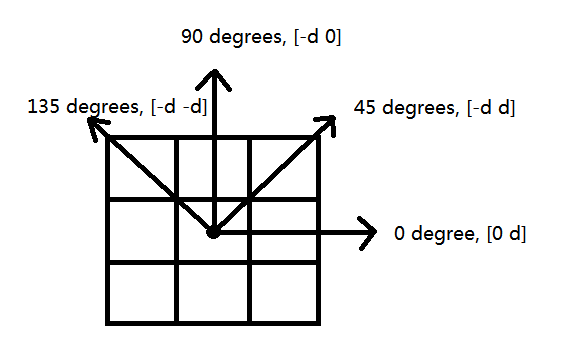
\includegraphics[width=1.3\headerheight]{offset}
        \captionof{figure}{Offsets used for different matrix}
        \label{fig:figlabel}
    \end{center}

  \end{itemize}
\end{itemize}


\end{posterbox}






\begin{posterbox}[name=accuracy,column=1,below=feature,above=bottom]{Accuracy of Classification}

\begin{center}
  \begin{tabular}{|c|c|c|}
    \toprule
      & Splitting & No Splitting\\
    \midrule
    accuracy & 96.0\% & 94.9\%\\
    \bottomrule
  \end{tabular}
  \captionof{table}{Accuracy of SVM based on HOG features}
  \label{tab:tablabel}
\end{center}

\begin{center}
  \begin{tabular}{|c|c|c|c|c|c|c|}
    \toprule
     step &1&2&3&4&5&6\\
    \midrule
    accr & .86 & .87 & .882 & .897 & .899 & .90\\
    \bottomrule
  \end{tabular}
  \captionof{table}{Accuracy of SVM based on co-occurrence matrix features}
  \label{tab:tablabel}
\end{center}



\end{posterbox}







\begin{posterbox}[name=experiment,column=2,below = example]{Experiment}
We use dataset with about 1000 pictures from International Conference on Document Analyze and Recognition (ICDAR) to train and test.

\begin{center}
  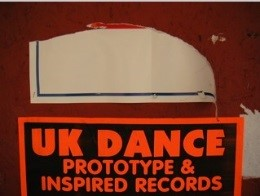
\includegraphics[width=1\headerheight]{ex11.jpg}
  
\includegraphics[width=1\headerheight]{ex12.jpg}
  \vspace{0.15cm}
  \hfill
  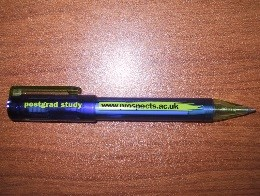
\includegraphics[width=1\headerheight]{ex21.jpg}
  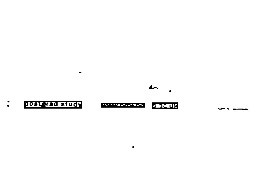
\includegraphics[width=1\headerheight]{ex22.jpg}
  \vspace{0.15cm}
  \hfill
  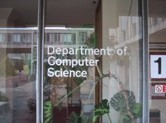
\includegraphics[width=1\headerheight]{ex31.jpg}
  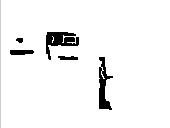
\includegraphics[width=1\headerheight]{ex32.jpg}
  \captionof{figure}{Good and bad examples}
  \label{fig:figlabel}
\end{center}

\end{posterbox}








\begin{posterbox}[name=future,column=2,below=experiment]{Future Work}
  \begin{itemize}
    \item Unsupervised Feature Learning also known as Deep Learning gives a promising way to find intrinsic feature of text pattern.
    \item Try to use a more efficient detection strategy like classifier cascade.
  \end{itemize}
\end{posterbox}











\begin{posterbox}[name=ackn,column=2,below=future,above=bottom]{Acknowledgements}
The author acknowledge resourceful discussion and support from professors and students from Key Lab. of Machine Perception (MoE),without whom this work would never have been started and finished.

\end{posterbox}

\end{poster}
\end{document}
